\iffalse
Noether's theorem says that continuous symmetries of physical systems gives rise to conservation laws. In this class we'll see some examples of low dimensional Lie groups and how they give rise to various phenomenon in physics like time dilation and length contraction in special relativity, spin states of electrons.

Keywords: bilinear forms, signature, SO(2), SO(3), Spin, SO(1,3), Minkowski space and relativity, Noether's theorem, Lie groups.

Prereqs: Linear algebra, Group theory
Homework: Recommended
\fi



\documentclass{article}
\usepackage{amsmath, amsthm}
\usepackage{amssymb}
\usepackage{mathtools}
\usepackage[all,cmtip]{xy}
\usepackage{color}


\setcounter{tocdepth}{4}

\renewenvironment{proof}{ {\bfseries Proof:}}{\qed}

\newtheoremstyle{mytheorem}%                % Name
{}%                                     % Space above
{}%                                     % Space below
{\itshape}%                                     % Body font
{0pt}%\parindent}%                                     % Indent amount
{\bfseries}%                            % Theorem head font
{.}%                                    % Punctuation after theorem head
{ }%                                    % Space after theorem head, ' ', or \newline
{}%                                     % Theorem head spec (can be left empty, meaning `normal')

\theoremstyle{mytheorem}
\newtheorem{thm}{Theorem}[section]
\newtheorem{proposition}[thm]{Proposition}
\newtheorem{lemma}[thm]{Lemma}
\newtheorem{corollary}[thm]{Corollary}


\newtheoremstyle{mydefinition}%                % Name
{}%                                     % Space above
{}%                                     % Space below
{}%                                     % Body font
{0pt}%\parindent}%                                     % Indent amount
{\bfseries}%                            % Theorem head font
{.}%                                    % Punctuation after theorem head
{ }%                                    % Space after theorem head, ' ', or \newline
{}%                                     % Theorem head spec (can be left empty, meaning `normal')

\theoremstyle{mydefinition}
\newtheorem{definition}[thm]{Definition}
\newtheorem{example}[thm]{Example}
\newtheorem{exercise}[thm]{Exercise}
\newtheorem{remark}[thm]{Remark}
%\newtheorem{ques}[thm]{Q.}
\newtheorem*{ques}{Question}
%\newtheorem{ans}[thm]{Ans.}
\newtheorem*{ans}{Ans}



\numberwithin{equation}{section}

%Real numbers, complex numbers, etc.
\newcommand{\R}{\mathbb{R}}
\newcommand{\C}{\mathbb{C}}
\newcommand{\Z}{\mathbb{Z}}
\newcommand{\Q}{\mathbb{Q}}
\renewcommand{\P}{\mathbb{P}}

%How does latex not have these?
\DeclareMathOperator{\Ad}{Ad}
\DeclareMathOperator{\ad}{ad}
\DeclareMathOperator{\tr}{tr}
\DeclareMathOperator{\Tr}{Tr}
\DeclareMathOperator{\Hom}{Hom}
\DeclareMathOperator{\Spec}{Spec}
\DeclareMathOperator{\im}{im}
\DeclareMathOperator{\rank}{rank}
\DeclareMathOperator{\Exists}{\exists}
\DeclareMathOperator{\Forall}{\forall}

\DeclareMathOperator*{\colim}{colim}
\DeclareMathOperator*{\holim}{holim}
\DeclareMathOperator*{\hocolim}{hocolim}


%fractions and inner product
\newcommand{\pr}[2][\:]{\frac{\partial #1}{\partial #2}}
\newcommand{\innerp}[2]{\langle #1, #2 \rangle}

\newcommand*\conj[1]{\overline{#1}}
\newcommand*\norm[1]{\lVert #1 \rVert}

\renewcommand{\figurename}{Fig.}
\usepackage{float}
\usepackage{wrapfig}

\usepackage{enumitem}
\setlist[enumerate]{itemsep=0mm}
\usepackage{geometry}
\geometry{
	a4paper,
	total={170mm,257mm},
	left=20mm,
	top=20mm
}


\usepackage{fancyhdr}
\pagestyle{fancy}
\lhead{\scshape Apurva Nakade}
%\rhead{\scshape Mathcamp 2017}
\renewcommand*{\thepage}{\small\arabic{page}}

\DeclareMathOperator{\re}{Re}



\begin{document}
\title{How to define a Square Root}
\author{Apurva Nakade}
\thispagestyle{fancy}
\maketitle




\section{Introduction}

The goals of this class are the following:
\begin{enumerate}
	\item Define inverses of complex differentiable functions
	\item Understand how it naturally leads to the definition of Riemann surfaces
	\item Define Riemann surfaces using implicit functions of the form $f(w,z) = c$
	\item Study branched coverings of Riemann surfaces.
\end{enumerate}

While trying to define inverses of complex differentiable functions $w = f(z)$ and more generally solution sets of functions of the form $f(z,w)=0$ Riemann stumbled upon the notion of a Riemann surface. Riemann surfaces are complex manifolds built out of gluing pieces of the complex plane, the subtlety lies in the way in which complex analysis is used to glue the pieces.

\textbf{Disclaimer:} This is not a complex analysis class so for the sake of lucid exposition there will be arguments which are not rigorous but which can be made rigorous by adding a few $\epsilon's$ and $\delta's$. It would be a very good exercise to work out these details by yourselves.\\

The square root function on real numbers $x \mapsto \sqrt{x}$ is defined as an inverse of the square function $f(x) = x^2$. In order for this to be well defined we need to restrict the domain to $x \ge 0$. Further we have to make a choice between the two possible values of $\sqrt{x}$.

While this is a reasonable thing to do for $\sqrt{x}$, this solution does not work too well for more complicated functions. Say we wanted to define the inverse function of the polynomial $f(x) = x(x-1)(x+1)$. Which domain should we pick and what should be the appropriate inverse? We need to make an arbitrary choice in each region where $f(x)$ is strictly increasing or decreasing and that is pretty much the end of the story.


\section{Complex numbers make things worse}
Recall that every complex number $z$ can be written as $z = r e ^{i \theta}$ where $r$ is the distance of $z$ from the origin and $\theta$ is the angle $z$ makes with the real axis in the counter clockwise direction. There is a natural way to extend the square root function to complex numbers using the polar decomposition of complex numbers.

\begin{align}
	\sqrt{z} : \C  & \rightarrow \C                                                          \\
	r e^{i \theta} & \mapsto \sqrt{r}.e^{i \theta/2} \qquad \mbox{ for } \theta \in [0,2\pi)
\end{align}

However this function is not continuous. If we think of the argument $\theta$ as varying from $0$ to $2 \pi$ then the function $\sqrt{z}$ as defined above is discontinuous at $\theta = 2 \pi$. As with real numbers there is another way to define the square root function,

\begin{align}
	\sqrt{z} : \C  & \rightarrow \C                                                           \\
	r e^{i \theta} & \mapsto -\sqrt{r}.e^{i \theta/2} \qquad \mbox{ for } \theta \in [0,2\pi)
\end{align}
This function also has a discontinuity at $\theta = 0$. We can also change where the discontinuity occurs by redefining the range for $\theta$
\begin{align}
	\sqrt{z} : \C  & \rightarrow \C                                                            \\
	r e^{i \theta} & \mapsto \sqrt{r}.e^{i \theta/2} \qquad \mbox{ for } \theta \in [-\pi,\pi)
\end{align}

The first solution to the above conundrum is analytic. Just like we did for the real numbers we try to define an inverse function in the largest possible domain of the complex numbers.

Consider the first definition of the function $\sqrt{z}$. The only place where this function is discontinuous is when $\theta = 0$, so we have a well defined square root on the open set $\theta \neq 0$ and we can define a square root on the complement
\begin{align}
	\sqrt{z} : \C \setminus \{ \theta = 0\} & \rightarrow \C                  \\
	r e^{i \theta}                          & \mapsto \sqrt{r}.e^{i \theta/2}
	\qquad \mbox{ for } \theta \in (0,2\pi)
\end{align}
This is a less than ideal solution as we probably do want the square root function to be defined on positive real numbers. One way to remedy this is to change the range of $\theta$
\begin{align}
	\sqrt{z} : \C \setminus \{ \theta = \pi\} & \rightarrow \C                                                            \\
	r e^{i \theta}                            & \mapsto \sqrt{r}.e^{i \theta/2} \qquad \mbox{ for } \theta \in (-\pi,\pi)
\end{align}


\subsection{Branch points and Branch cuts}
\begin{definition}
	Removing the ray $\theta = \pi$ or the ray $\theta = 0$ is an example of a \textbf{branch cut} for the function $\sqrt{z}$. Say we make a cut $\theta = \pi$ and let $\theta$ vary between $(-\pi, \pi)$ then the possible functions $\sqrt{r}.e^{i \theta/2}$ and $-\sqrt{r}.e^{i \theta/2}$ are called \textbf{branches} of the function $\sqrt{z}$.
\end{definition}
It is more generally possible to remove \textbf{any} curve starting at the origin that escapes to $\infty$ and choose a branch of $\sqrt{z}$ on the complement, for example if we have a curve $\theta = \phi(r)$ in the polar coordinates then the following is a possible branch of $\sqrt{z}$,

\begin{align}
	\sqrt{z} : \C \setminus \{ \theta = \phi(r)\} & \rightarrow \C                                                     \\
	r e^{i \theta} & \mapsto \sqrt{r}.e^{i \theta/2} &
\end{align}
where the range of $\theta$ is now a function of $r$ as $\theta \in (-\pi - \phi(r),\pi - \phi(r))$. The curve escaping to $\infty$ does not have to be of the form $\theta = \phi(r)$ (see Exercise \ref{thm:ex1}).

How does this generalize to other polynomials? Consider the polynomial $f(z) = z^n$ for a positive integer $n$. Just as we had two branches for $\sqrt{z}$ we have $n$ branches of the function $z^{1/n}$ one for each integer $n^{th}$ root of unity. For $0 \le k < n$ we can define $n$ branches of $z^{1/n}$ as follows,
\begin{align}
	z^{1/n} : \C \setminus \{ \theta = \pi\} & \rightarrow \C                                                     \\
	r e^{i \theta} & \mapsto {r}^{1/n}.e^{i \theta/n}.e^{2 \pi k i/n} & \mbox{ for } \theta \in (-\pi,\pi)
\end{align}
We'll see how to generalize this for more general polynomials later.




\section{Complex numbers make things better}
Riemann's idea was to not make a choice at all and glue all the branches of the function together. For the branch cut $\theta = \pi$ the two branches of the function $\sqrt{z}$ are
\begin{align}
	\sqrt{r e^{i\theta}} = \sqrt{r} e^{i\theta/2} \quad \mbox{ and } \quad \sqrt{r e^{i\theta}} = -\sqrt{r} e^{i\theta/2}
\end{align}
These two branch cuts are not independent of each other but one is naturally a continuation of the other and we can glue the two together to get an even larger domain on which the square root function can be defined.

Suppose that we've two different complex planes $\C$ with branch cuts, on each we apply the two branch functions. If we imagine traversing the unit circle in the counterclockwise direction on both the planes starting and ending at $-1$ and applying the two branch cuts of $\sqrt{z}$, then as we \emph{finish} the loop on the first the value of the first branch function approaches $i$ and as we \emph{start} the second loop the branch function approaches the value $i$. If we glue the two accordingly we get our first \textbf{Riemann surface}

\begin{figure}[H]
	\centering
	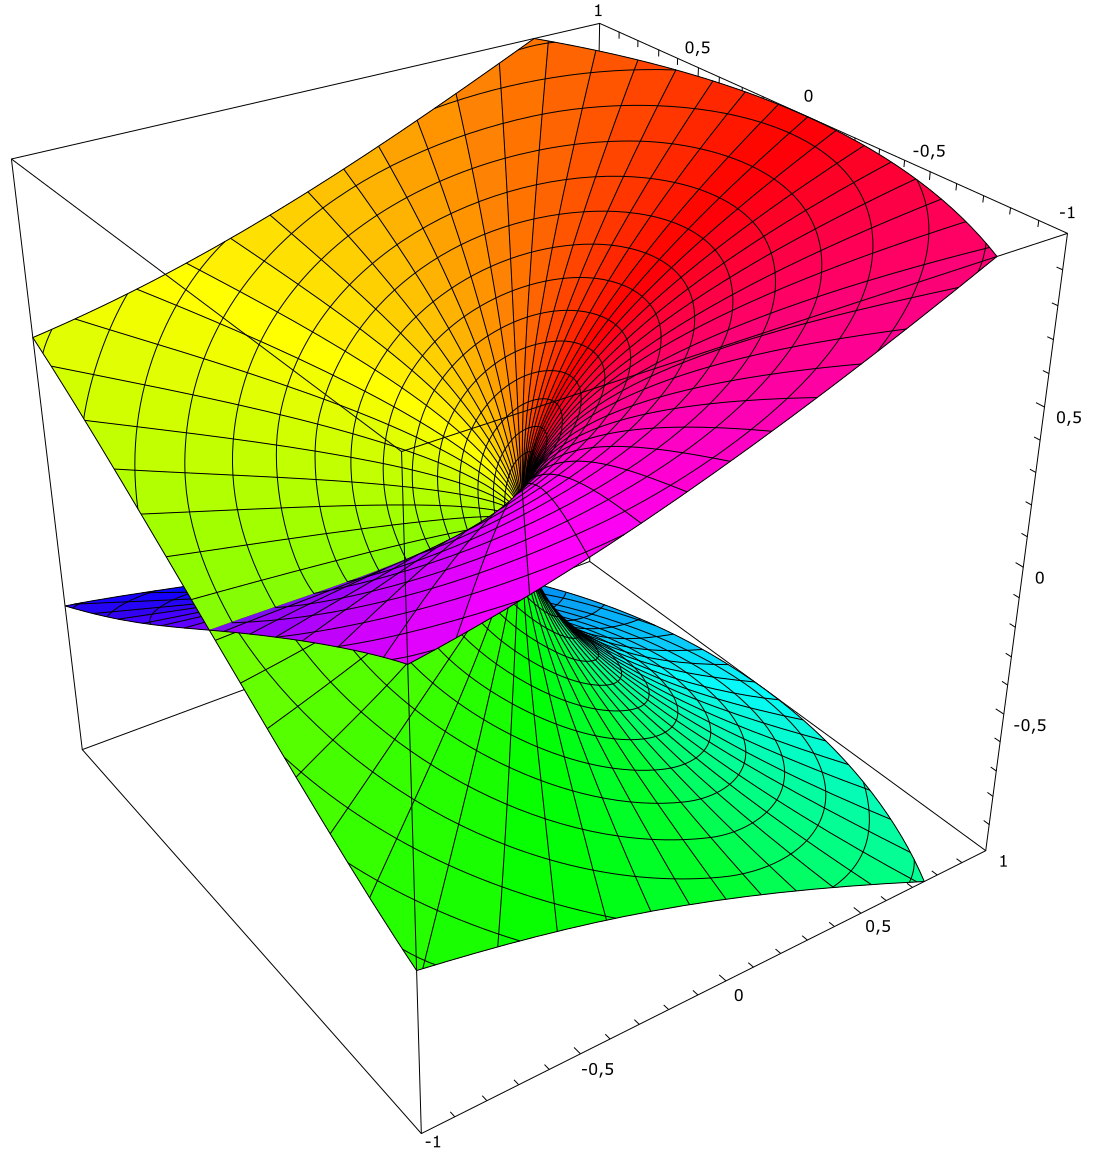
\includegraphics[width=0.35\linewidth]{images/sqrt}
	\caption{Riemann Surface on which the square root is properly defined}
	\label{thm:img1}
\end{figure}

On this Riemann surface the function $\sqrt{z}$ is well defined and it's image is the entire complex plane $\C$. Note that even though in Figure.\ref{thm:img1} the surface appears to be intersecting itself, but that is only because of our inability to represent more than 3 dimensions on paper. As a \emph{topological space} the Riemann surface has no self intersections. This is made rigorous by defining the Riemann surface as a complex manifold i.e. a manifold that locally looks like the complex plane.

We can similarly define Riemann surfaces for the functions $z^{1/n}$. For these we need to glue $n$ copies of the complex plane with a branch cut appropriately.\\
\begin{center}
	\begin{tabular}{ccc}
		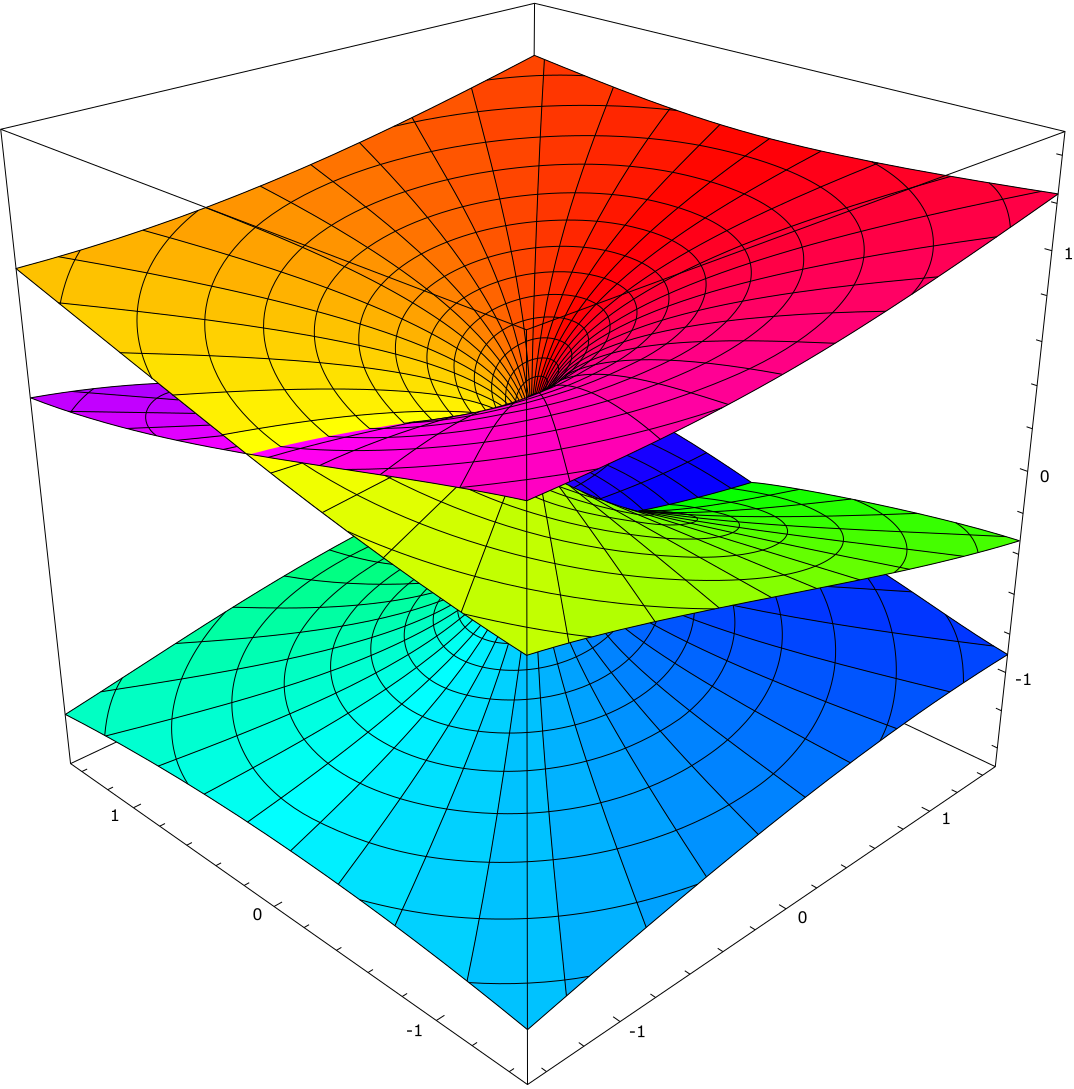
\includegraphics[width=0.35\linewidth]{images/cube_root} & $\qquad$ &
		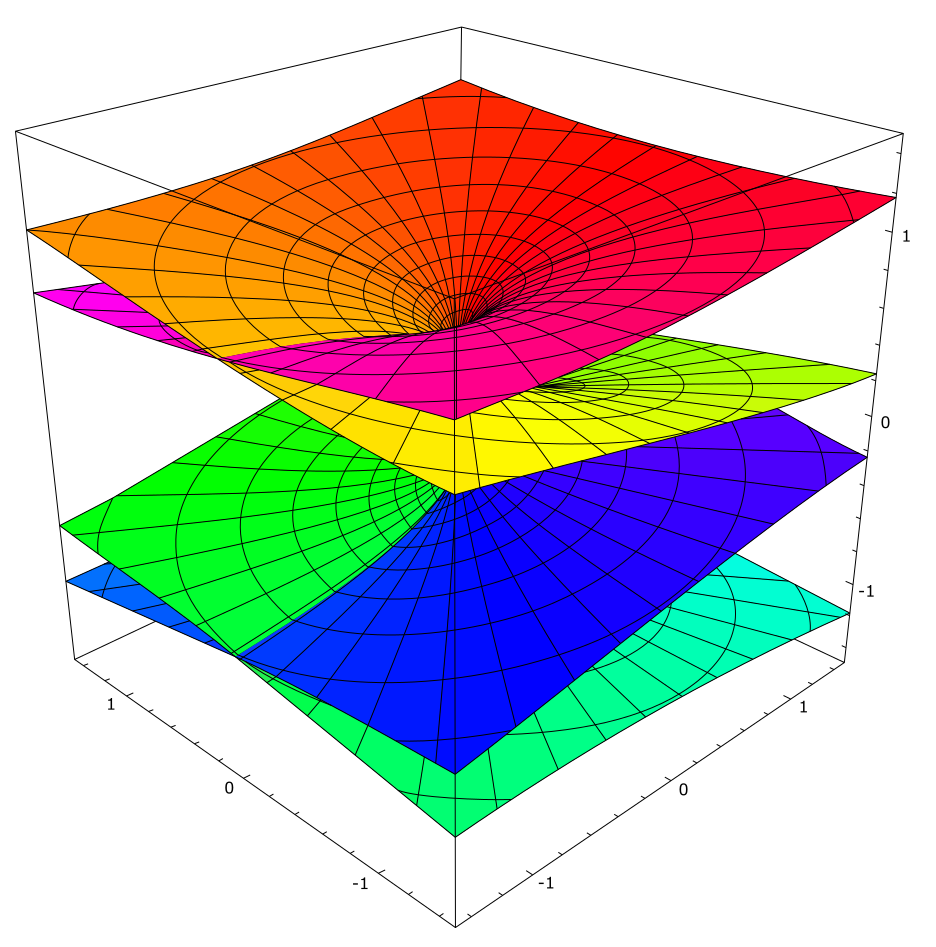
\includegraphics[width=0.35\linewidth]{images/4th_root} \\
		$z^{1/3}$                                                &          & $z^{1/4}$
	\end{tabular}
\end{center}



\section{Exercises}

\begin{exercise}
	\label{thm:ex1}
	For any branch cut for $\sqrt{z}$ there are exactly two possible branch functions. Can you prove this rigorously?
\end{exercise}

\begin{exercise}
	Find some branch cuts, corresponding branches and resulting Riemann surface for the following functions. Describe the images of the Riemann surfaces under the corresponding functions $f(z)$.
	\begin{enumerate}
		\item $f(z) = {z-1}$
		\item $f(z) = \sqrt{z-1}$
		\item $f(z) = \sqrt{z-1}+1$
		\item $f(z) = \log z$
	\end{enumerate}
\end{exercise}

\begin{exercise}
	Is the following curve a valid branch cut for $\sqrt{z}$? What could be a branch for $\sqrt{z}$ on this domain?
	\begin{figure}[H]
		\centering
		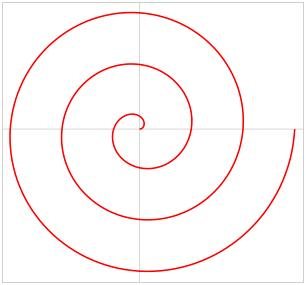
\includegraphics[width=0.25\linewidth]{images/spiral}
		\caption{Spiral}
	\end{figure}

\end{exercise}


\end{document}
